\chapter{Simulaci\'on de ebullici\'on en FC-72}

En los primeros cap\'itulos de esta tesis se introdujo, analiz\'o y valid\'o un modelo que permite reproducir adecuadamente una ecuaci\'on de energ\'ia para flujo multif\'asico, tomando como base una nueva \lbe{} con operador de colisi\'on MRT que debe ser resuelta en forma simult\'anea con otra \lbe{} hidrodin\'amica de la familia \pp{}. El desarrollo de este nuevo modelo no qued\'o restringido \'unicamente a la nueva ecuaci\'on y su justificaci\'on formal, sino que forma parte de una m\'etodolog\'ia de an\'alisis destinada a realizar simulaciones consistentes de transferencia de calor en flujo multif\'asico.

El nuevo modelo, en sus versiones D2Q9 y D3Q15, fue validado mediante la resoluci\'on de problemas en los que es posible obtener una soluci\'on anal\'itica. En estos \red{problemas}, en su mayor\'ia unidimensionales, fue posible discriminar diferentes aspectos de las ecuaciones macrosc\'opicas recuperadas, permitiendo desarrollar un an\'alisis de las \lbe{} desde un punto de vista global, que abarca aspectos fundamentales de las t\'ecnicas num\'ericas cl\'asicas como precisi\'on y consistencia. 

Esta metodolog\'ia de verificaci\'on consiste en un primer paso obligatorio en el proceso de validaci\'on de cualquier t\'ecnica num\'erica o modelo novedoso. Sin embargo, siempre que sea posible, este proceso debe completarse con la evaluaci\'on de situaciones m\'as complejas y que involucren una fenomenolog\'ia similar a la que se pretende resolver con la nueva t\'ecnica, tomando mediciones o resultados de simulaciones que puedan usarse para construir una base de comparaci\'on s\'olida.

En este aspecto, la representaci\'on de experimentos o simulaciones de ebullici\'on como parte de la validaci\'on resulta una tarea sumamente compleja. El modelo de lattice Boltzmann propuesto constituye un mecanismo alternativo para obtener la soluci\'on de ecuaciones diferenciales de conservaci\'on de masa, impulso y energ\'ia en flujo multif\'asico, y no involucra el modelado de caracter\'isticas microsc\'opicas del fen\'omeno de ebullici\'on que surgen de aquellos enfoques basados en las mayores escalas espaciales. Como de destaca en la extensa revisi\'on de Liang y Mudawar \cite{liang_review_2019}, la din\'amica de estos procesos no depende simplemente de las propiedades del fluido, sino que se encuentra fuertemente influenciada por las caracter\'isticas microsc\'opicas de la superficie calefactora. De esta manera, los aspectos macrosc\'opicos m\'as representativos, como temperatura o flujo de calor en la superficie, o tama\~no de las burbujas, presentan una fuerte dependencia con la cantidad y forma de los sitios de nucleaci\'on, porosidad y permeabilidad de la superficie, tensi\'on superficial y \'angulo de contacto. Por lo tanto, esta fuerte dependencia dificulta la selecci\'on de experimentos que puedan ser usados como casos de validaci\'on, ya que en muchas ocaciones no es posible determinar a priori estas propiedades que deben ser reproducidas num\'ericamente.

A pesar de estas restricciones inherentes al fen\'omeno, en los \'ultimos a\~nos se produjo un avance significativo en el desarrollo de microdispositivos para levar a cabo experimentos de ebullici\'on, permitiendo un notable control sobre los sitios de nucleaci\'on. De esta manera, la incorporaci\'on de sensores exclusivamente en la zona de generaci\'on de las burbujas y el uso de c\'amaras de alta velocidad y resoluci\'on, permitieron lograr una reconstrucci\'on detallada de procesos elusivos, como la formaci\'on, crecimiento y desprendimiento de burbujas individuales. En este l\'inea, Hutter y colaboradores \cite{hutter_experimental_2009,hutter_experimental_2010} lograron medir experimentalmente di\'ametro de burbujas en funci\'on del tiempo, frecuencia, di\'ametro de partida y tiempo de espera, en la ebullici\'on de FC72 sobre obleas de silicio con un n\'umero reducido de cavidades microfabricadas. 

Las caracter\'isticas de estas mediciones, en las que se reducen las incertezas asociadas a la descripci\'on de la superficie y se logra determinar con precisi\'on aquellas caracter\'isticas del flujo reproducibles con lattice Boltzmann, las convierten en un caso de validaci\'on ideal para el modelo propuesto en esta tesis. Por lo tanto, el presente cap\'itulo estar\'a dedicado a la reproducci\'on del experimento de ebullici\'on de Hutter mediante la aplicaci\'on del modelo y de la metodolog\'ia de an\'alisis desarrollada en los cap\'itulos anteriores.




\section{Descripci\'on del experimento}

El cuerpo principal del dispositivo experimental de Hutter \cite{hutter_experimental_2010} est\'a compuesto por una c\'amara de ebullici\'on de acero inoxidable, con cuatro ventanas de vidrio \red{borosilicato}, que permiten el acceso \'optico al substrato de ebullici\'on. Esta c\'amara se encuentra recubierta con calefactores aislados con silicona que permiten reducir la p\'erdida de calor hacia el ambiente, y contiene cuatro cartuchos calafactores utilizados para la desgasificaci\'on del \red{boiling l\'iquid} y para calefaccionarlo hasta alcanzar la temperatura de saturaci\'on. La c\'amara se encuentra conectada a un condensador externo, el cual es responsable de regular la presi\'on del sistema mientras que permite la recuperaci\'on del l\'iquido evaporado y su posterior regreso a la c\'amara principal.

El componente responsable de la ebullici\'on consiste en un chip de silicio, construido sobre una oblea de 3 pulgadas de di\'ametro y 380 $\mu m$ de espesor. En la \fig{fig:chip} se esquematiza el proceso de construcci\'on del chip: en uno de sus caras se produce una capa de di\'oxido de silicio que contiene en su interior a los sensores de temperatura y el circuito calefactor de Al, mientras que en la superficie restante se generan las microcavidades que actuar\'an como sitios de nucleaci\'on.

\begin{figure}[ht]
	\centering
	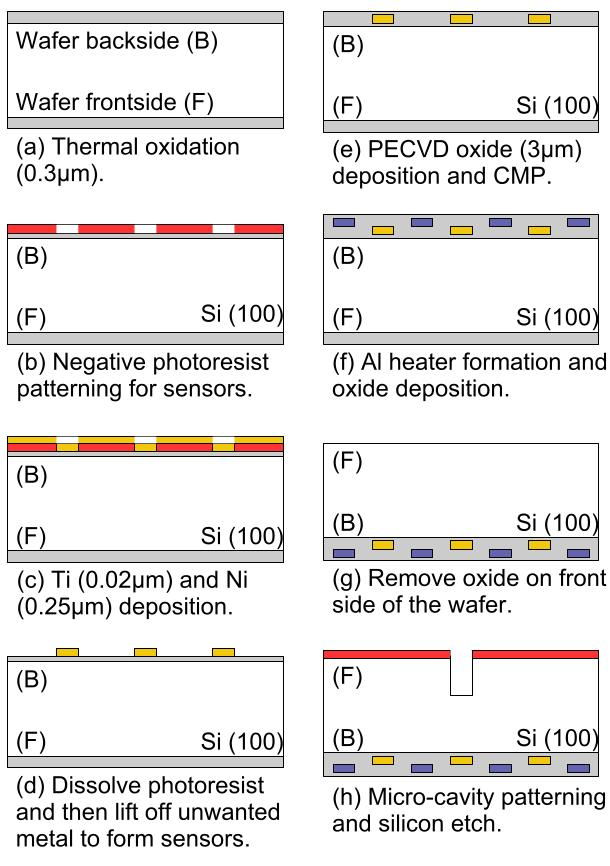
\includegraphics[width=0.5\textwidth]{FC72/Substrate}
	\caption{Secuencia de fabricaci\'on del chip de ebullici\'on, que contiene las microcavidades, los sensores de temperatura integrados (amarillo), y la resistencia calefactora integrada (azul). Reimpreso de \cite{hutter_experimental_2010}.}
	\label{fig:chip}
\end{figure}

Las cavidades artificiales fueron generadas sobre la placa de silicio mediante un proceso de grabado profundo con iones activos (\emph{deep reactive ion etching}), y corresponden a peque\~nos orificios de 40 $\mu m$ de profundidad y 10 $\mu m$ de di\'ametro. Como se muestra en la \fig{fig:cavidad}, esta t\'ecnica permite generar cavidades con formas precisas, claramente distinguibles de la rugosidad superficial del chip.

\begin{figure}[ht]
	\centering
	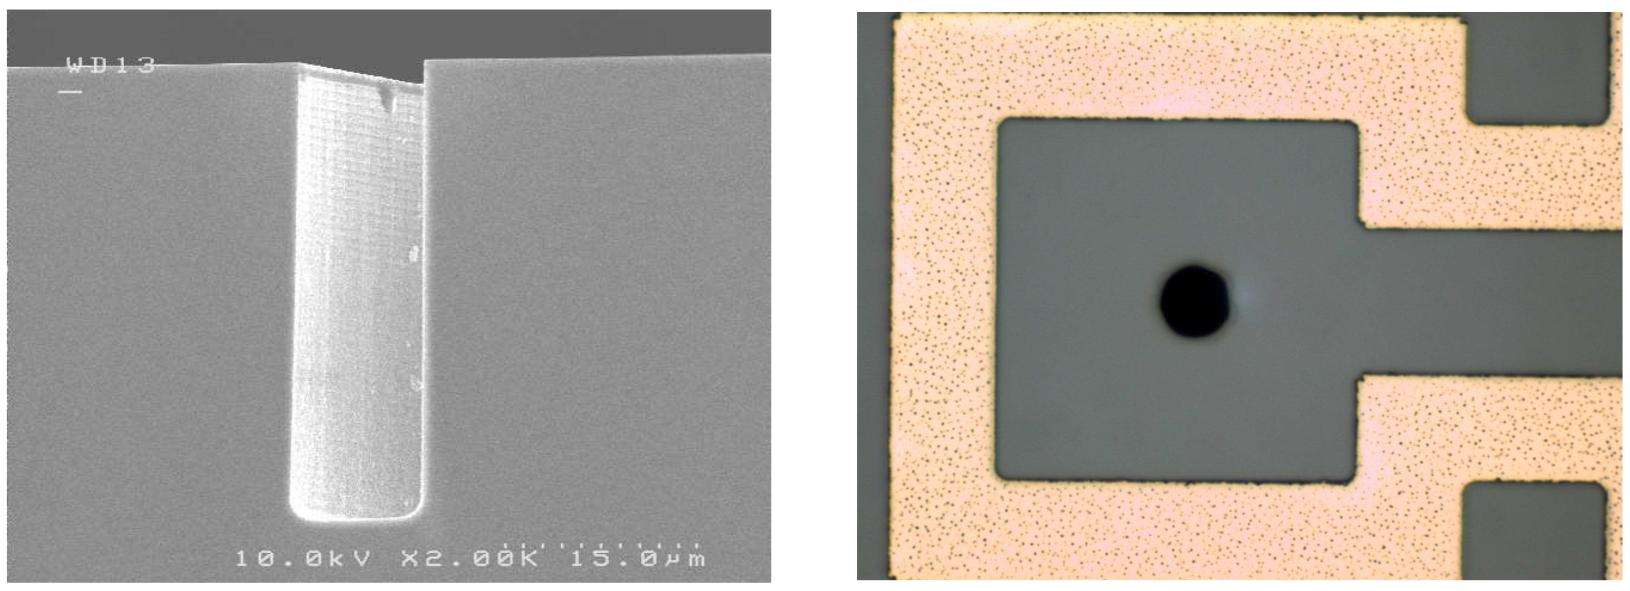
\includegraphics[width=0.75\textwidth]{FC72/Cavity}
	\caption{Izquierda: imagen SEM de una secci\'on a trav\'es de una cavidad elongada. Derecha: imagen de la apertura de la cavidad.}
	\label{fig:cavidad}
\end{figure}


\subsubsection{\red{Boiling liquid}}

El fluido de trabajo utilizado fue perfluorohexano C$_6$F$_14$, conocido comercialmente como Fluorinert FC-72. Es un l\'iquido claro, incoloro, t\'ermica y qu\'imicamente estable, compatible con materiales sensibles, inflamable, poco t\'oxico y ampliamente utilizado en experimentos de ebullici\'on. Su baja temperatura de ebullici\'on ($T_{sat}=57.15$ \textordmasculine C a 1 atm de presi\'on) y sus propiedades diel\'ectricas permiten sumergir completamente las conexiones el\'ectricas de la c\'amara y el chip calefactor.  \red{Algo m\'as}


El di\'ametro de las burbujas pudo ser medido a partir de im\'agenes capturadas por una c\'amara de alta velocidad, y corresponde al m\'aximo di\'ametro aparente o ecuador de las mismas. En la \fig{fig:sequence} se muestra una secuencia de im\'agenes con una resoluci\'on temporal de 6 ms para el crecimiento de una burbuja en una cavidad de 80 $\mu$m de profundidad y 10 $\mu$m de di\'ametro, con un exceso de temperatura de 1.1 K en la superfcie calefactora (respecto a la temperatura de saturaci\'on) y 1.25 atm de presi\'on.

\begin{figure}[ht]
	\centering
	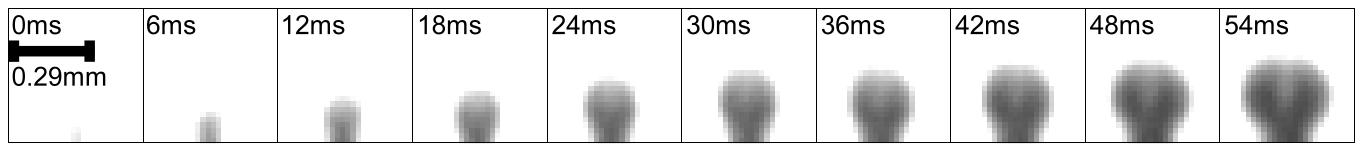
\includegraphics[width=0.9\textwidth]{FC72/sequence}
	\caption{Im\'agenes de alta velocidad de la secuencia de crecimiento de una burbuja en una cavidad aislada.}
	\label{fig:sequence}
\end{figure}





\section{Modelo num\'erico}